\vspace{10pt}

\minitoc
\clearpage

\section{Introduction}
%On présente dans cette partie quelques observations liées à l'exécution de l'ensemble de l'algorithme proposé dans les étapes précédentes. Les problématiques de temps de calcul sont abordées dans un premier temps, ainsi que des exemples de résultats obtenus sur plusieurs jeux de données, que l'on présente ici à titre d'illustration.

Dans l'objectif d'évaluer les performances de l'approche présentées dans cette thèse, nous avons procédé à des expérimentations et évaluations exhaustives sur des séquences issues de bases de données variées, provenant de de benchmarks différents. Dans un premier temps, nous voulons  aborder le problème classique du temps de calcul. Ensuite, nous présentons des résultats obtenus sur plusieurs jeux de données. Il aurait été intéressant néanmoins de tester nos algorithmes sur des bases de données simulées afin d'évaluer la pertinence des démarches dans des cas réalistes idéaux. Malheureusement, nous ne disposons pas de tels bases de données et n'avons pas connaissance de l'existence de telles bases dans la communauté \footnote{Il aurait cependant été possible d'utiliser des données simulées, telles que celles rendues possibles par le simulateur CIVIC. Nous nous en sommes tenus à des données réelles, mais ne disposant alors pas de vérité terrain.}. Les résultats présentés sont donc essentiellement qualitatifs.

\section{Temps de calcul}\label{sec:ch6_temps_reel}
\subsection{Coût des différentes étapes}
\paragraph{Exemple de répartition:\\}
Nous recensons dans le tableau \ref{tab:ch6_temps_de_calcul} les temps de calcul moyens des différentes étapes algorithmiques du diagramme de fonctionnement présenté dans la figure \ref{fig:ch2_approche_proposée}. Nous avons vu dans les sections précédentes (notamment \ref{sec:ch3_Implémentation}, \ref{sec:ch4_temps_de_calcul} et \ref{sec:ch5_temps_de_calcul}) que le temps d'exécution de ces processus était variable, et la répartition présentée ici ne concerne que des valeurs moyennes. Les principaux paramètres correspondant sont : 4000 points suivis par paire d'images, images rectifiées de taille 1240 x 370, utilisation de 80 acquisitions consécutives pour filtrer les résultats.	La figure \ref{fig:ch6_repartition_calcul} représente graphiquement la répartition approximative du coût calculatoire des différentes étapes de l'algorithme proposé. 

\begin{figure}
	\centering
	\includegraphics[width=0.98\textwidth]{Chapter6/graphics/repartition_temps_calcul.png}
	\caption{Répartition du temps de calcul des différentes étapes}
	\label{fig:ch6_repartition_calcul}
\end{figure}

\begin{figure}
	\renewcommand{\arraystretch}{1.2}
	
	\begin{equation}
	\begin{array} {| c | c |}
	\hline
	\textnormal{Étape} & \textnormal{Temps de calcul (ms)} \\
	\hline
	\textnormal{Détection des points} 									& 8 	\\
	\textnormal{Suivi des points} 											& 45 	\\
	\textnormal{Estimation de l'ego-motion}							& 1,5		\\
	\textnormal{Reconstruction de l'environnement} 			& 25		\\
	\textnormal{Détection et suivi des objets mobiles} 	& 40		\\
	\hline
	\textnormal{Temps total} & 119,5\\
	\hline
	\end{array}
	\end{equation}
	\caption{Temps de calcul moyens}
	\label{tab:ch6_temps_de_calcul}
\end{figure}

\paragraph{Remarques:\\}
% Enseignements sur du temps à gagner par endroits ?
On pourra tout d'abord constater que les trois grandes étapes du calcul (suivi des points dans l'espace image, reconstruction de l'environnement en trois dimensions, détection et suivi des objets mobiles) sont relativement équitablement réparties. Une amélioration du temps de calcul nécessaire à l'algorithme n'est donc pas triviale, et doit considérer l'ensemble de ces étapes.\\

Deux paramètres permettent d'influer sur ce temps de calcul, et ont un impact différent sur les différentes parties de l'algorithme. \\
Il est tout d'abord possible de conserver plus ou moins d'acquisitions en mémoire. L'augmentation de ce nombre peut améliorer la précision des points positionnés, le sur-échantillonnage (observations multiples de la position d'un même point) améliorant de manière assez classique le rapport signal/bruit. Cela permet ensuite d'agrandir l'environnement \og connu\fg{}, dans le cas où le porteur se déplace, ce qui peut être une conséquence recherchée. La variation du temps de calcul en fonction du nombre d'acquisitions conservées est dans ce cas approximativement linéaire, deux régimes étant cependant possibles : le nombre d'acquisitions est de l'ordre du temps de présence des indices visuels dans l'image, ou bien très supérieur \footnote{Comme nous l'avons vu dans la section \ref{sec:ch4_filtrage_des_points}, trois régimes sont possibles dans l'estimation de la position des points d'intérêts. Si ceux-ci sont encore visibles, ils peuvent être statiques ou mobiles, auquel cas leur position est estimée à chaque nouvelle observation selon un procédé différent. Si ces points ne sont plus visibles, leur dernière position connue est reportée dans le référentiel courant, ce qui est moins coûteux. La variation du temps de calcul en fonction du nombre d'observations prises en compte suit donc ces deux coûts marginaux différents.}. Ce paramètre influe finalement sur les parties \og 3D\fg{} de l'algorithme, et pas sur la partie visuelle.\\
Un deuxième paramètre consiste à ajuster le nombre de points suivi par paire d'images acquises. Ce peut être un moyen d'augmenter la probabilité de détection des objets mobiles, d'améliorer la précision de l'estimation du mouvement, ou plus simplement de densifier la reconstruction de l'environnement. Ce paramètre modifie principalement le temps de calcul lié à la détection et au suivi de points, et peut empiriquement être compris entre 2000 et 8000 points par paire d'images selon les capacités de calcul présentes.\\

\subsection{Vitesse d'exécution}
\subsubsection{Latence et cadence d'exécution}
Dans ce paragraphe, on précise simplement les notions de latence et de cadence d'exécution, qui seront exploitées dans les sections suivantes. Ces notions sont certainement connues par le lecteur, il ne s'agit que d'une précision.

\begin{itemize}
	\item{\emph{Latence:\\}}
	On définit dans notre cadre d'exécution la latence par le temps entre l'acquisition des paires d'images (considéré comme un événement ponctuel) et la mise à disposition d'informations utiles.\\
	
	\item{\emph{Cadence:\\}}
	On définit par ailleurs la cadence comme la fréquence à laquelle les acquisitions peuvent être traitées en régime continu.\\
\end{itemize}
Dans le cas d'un algorithme purement séquentiel et monobloc la latence et la cadence sont bien sûr liées, mais cela n'est pas nécessairement le cas lorsque l'algorithme est morcelé et que des exécutions concurrentes sont possibles.

\subsubsection{Exécution en parallèle de deux parties séquentielles}
\paragraph{Introduction:\\}
% Parler du cas général
Lorsqu'un algorithme peut être décomposé en deux parties dont l'exécution est strictement séquentielle (c'est à dire que la seconde partie fonctionne à partir des résultats de la première mais ne déclenche pas de nouveaux calculs au sein de celle-ci), il est possible d'en accélérer la cadence d'exécution en acceptant d'en augmenter légèrement la latence.\\ Supposons que son temps de calcul global soit noté $\tau$, et que les temps d'exécution des parties 1 et 2 soient respectivement $\tau_1$ et $\tau_2$. Une exécution \og classique\fg{}, séquentielle, implique qu'une nouvelle donnée ne peut être traitée avant que l'ensemble de l'algorithme ait été exécuté, soit une cadence de $\frac{1}{\tau}$. En généralisant le raisonnement, et en notant $F$ la cadence d'exécution:
\begin{align}
	F_{seq} &= \frac{1}{\sum\limits_{i=1}^{N} \tau_i } \\
	\tau_{seq} &= \tau = \sum\limits_{i=1}^{N} \tau_i 
\end{align}

Supposons que l'on considère maintenant une exécution concurrente des parties 1 et 2 de l'algorithme, qui ne peuvent, dans ce cas, être consacrées à la même acquisition (puisque la partie 2 utilise les résultats de la partie 1). La partie 1 peut exécuter les calculs nécessaires à l'acquisition $k$, tandis que la partie 2 est exécutée sur les résultats de l'acquisition $k-1$. On démontre facilement que la nouvelle cadence d'exécution est maintenant limitée par la partie la plus lente des deux (dans l'hypothèse où l'exécution est en régime constant). En généralisant, on peut écrire dans ce cas :
\begin{align}
	F_{sim} &= \frac{1}{\max\limits_{i=1:N} (\tau_i) } \\
	\tau_{sim} &= N \cdot \max_{i=1:N} (\tau_i)
\end{align}
Dans le cas de portions de l'algorithme strictement égales en termes de temps de calcul, et en supposant que l'on dispose d'autant d'unités d'exécution que nécessaire, on constate donc qu'une exécution simultanée augmente la cadence d'un facteur $N$ (nombre de portions considérées), sans que la latence ne soit affectée ( $N \cdot \max_{i=1:N} (\tau_i) = \tau$). Si les différentes parties de l'algorithme exécutées simultanément ne sont pas strictement égales en temps de temps d'exécution, le gain en termes de cadence est au prorata de la partie la plus lente, tandis que la latence est pénalisée (le calcul donne bien sûr $N \cdot \max_{i=1:N} (\tau_i) > \tau$). Ce phénomène est illustré sur la figure \ref{fig:ch6_concurrent_execution}.

\paragraph{Implémentation:\\}
% Montrer que cette notion s'appliquait bien à notre problème
La configuration de notre algorithme se prête bien à une exécution concurrente de ses deux parties principales, telle qu'expliquée dans le paragraphe précédent. Les temps de calcul nécessaires dans l'espace image (détection et suivi robuste de points d'intérêt) et dans l'espace en trois dimensions (estimation de l'ego-motion, reconstruction de la position des points dans l'espace, détection et suivi des points mobiles) sont en effet comparables. Cette répartition est illustrée sur la figure \ref{fig:ch6_image_3D}.

\begin{figure}
	\centerline {
		\includegraphics[width=1.1\textwidth]{Chapter6/graphics/repartition_image_3D.png}
	}
	\caption{Conséquences d'une exécution entrelacée des deux principales étapes du calcul}
	\label{fig:ch6_image_3D}
\end{figure}

% Exemple pratique
L'implémentation d'une exécution entrelacée des deux parties principales de l'algorithme proposé n'est pas très complexe en pratique, nécessitant simplement la présence d'une mémoire tampon intermédiaire. Ce tampon est pris en charge par le programme intermédiaire RTMaps, de l'entreprise \emph{Intempora}. Un diagramme comparant une exécution monolithe et une exécution concurrente des deux principales parties de l'algorithme est visible sur la figure \ref{fig:ch6_concurrent_execution}.

\begin{figure}
	\centerline {
 	\includegraphics[width=1.1\textwidth]{Chapter6/graphics/concurrent_execution.png}
 	}
 	\caption{Conséquences d'une exécution entrelacée des deux principales étapes du calcul}
	\label{fig:ch6_concurrent_execution}
\end{figure}

\paragraph{Conséquences expérimentales:\\}
Dans les jeux de données \og New College\fg{} et \og KITTI\fg{}, introduits dans la section suivante, l'application du principe précédent permet de s'approcher dans un cas d'une exécution temps réel, et dans l'autre d'y accéder aisément.\\
Le jeu de données \og New College\fg{} a en effet été acquis à la cadence de 20 images par seconde, cadence qui n'est pas atteinte sur notre plate-forme de test avec le nombre de points initialement visé \footnote{Plate-forme : PC portable, Intel Core i7 2GHz, détection et suivi de 4000 points par acquisition, filtrage de l'environnement sur 100 acquisitions soit 5 secondes}. Il est en effet possible lors de nos expérimentations d'exécuter l'ensemble des traitements à la cadence d'environ 16 images par seconde.\\
Le jeu de données KITTI a été acquis à la cadence de 10 images par seconde, et son rejeu est possible avec notre algorithme à la cadence de 14 images par seconde \footnote{De même que précédemment, on suit 4000 points par acquisition, et on considère une fenêtre d'intégration de 100 mesures. La vitesse de déplacement du porteur est plus importante tandis que la cadence d'acquisition est plus faible, ce qui nécessite d'augmenter le voisinage de suivi des points d'intérêt, et augmente la taille du nuage de points reconstruit.}, ce qui nous garanti un traitement en temps réel.

\section{Expérimentations} 
\subsection{New College}
\subsubsection{Conditions expérimentales}
Ce jeu de données a été introduit précédemment dans ce manuscrit (section \ref{sec:ch3_Eval_PI} notamment), et est précisément décrit dans \cite{Smith2009}. Nous ne rappelons ici que les caractéristiques principales. Le véhicule porteur est un bicycle dérivé d'un véhicule \emph{Segway}, illustré sur la figure \ref{fig:ch6_nc_setup} tirée de \cite{Smith2009}. La cadence d'acquisition est de 20Hz, les images brutes (non rectifiées) ayant une définition de 512*384 pixels en niveaux de gris. L'écart entre les deux caméras est de 12 cm. Les acquisitions ont été effectuées à Oxford, dans le parc de l'université \og New College\fg{}.

\begin{figure}
	\centerline {
		\includegraphics[width=0.5\textwidth]{Chapter6/graphics/new_college_setup.png}
	}
	\caption{Plate-forme support des acquisitions. Illustration tirée de \cite{Smith2009}}
	\label{fig:ch6_nc_setup}
\end{figure}

\subsubsection{Exemples de résultats}
\paragraph{Environnement 3D:\\}
De nombreuses illustrations sont possibles pour donner un aperçu de la qualité de la reconstruction de l'environnement, mais une évaluation quantitative est délicate. D'autres exemples sont visibles dans le paragraphe \ref{fig:ch6_kitti}. On illustre dans les figures suivantes des cas de figure particuliers.\\

%Effet du filtrage dans le temps
On peut constater sur la figure \ref{fig:ch6_nc_range} l'impact de la distance d'observation sur la précision du positionnement, et le filtrage continu effectué sur chacun des points. Les points les plus proches de la caméra ont été observés plus longtemps, et les dernières observations (à plus courte portée) sont plus précises. Leur position s'est affinée, comme l'illustre \og l'épaisseur\fg{} du mur, qui rend compte de la dispersion des mesures. À l'inverse, les points les plus lointains sont à la fois les plus récents (du fait de la trajectoire du porteur) et ceux les plus mal observés (du fait de leur distance et du faible écartement -12cm- des deux caméras), et le bruit est plus présent. 

\begin{figure}
	\centerline{
		\begin{tabular}  {c c}	
			\begin{tabular} {c}
				\begin{subfigure}{0.4\textwidth}
					\centering
					\includegraphics[width=\textwidth]{Chapter6/graphics/new_college_range_pict.png} 
					\caption{Vue caméra}
				\end{subfigure}	
				\\
				\begin{subfigure}{0.4\textwidth}
					\centering
					\includegraphics[width=\textwidth]{Chapter6/graphics/new_college_range_aerial.png} 
					\caption{Vue aérienne (source : \textit{Google Earth})}
				\end{subfigure}	
			\end{tabular}
			&
			\begin{subfigure}{0.5\textwidth}
				\includegraphics[width=\textwidth]{Chapter6/graphics/new_college_range_crop.png} 
				\caption{Nuage de points reconstitué et trajectoire récente}
			\end{subfigure}
		\end{tabular}
	}
	\caption{Influence de la distance sur la précision de la reconstruction}
	\label{fig:ch6_nc_range}
\end{figure}

\paragraph{Détection et suivi des objets mobiles:\\}
On présente dans les figures \ref{fig:ch6_NC_move_1}, \ref{fig:ch6_NC_move_2}, \ref{fig:ch6_NC_move_3} et \ref{fig:ch6_NC_move_4} le résultat de notre algorithme de perception des objets mobiles dans le jeu de données \og New College\fg{}. D'autres cas de détections étaient présentés dans la section \ref{sec:ch5_exemple}, l'ensemble des objets mobiles visibles étant alors représenté.\\
Les seuls éléments de la scène étant en mouvement sont des piétons, mais cette information n'est pas prise en compte par notre proposition, comme illustré par la figure \ref{fig:ch6_KITTI_move}. La détection et le suivi des objets mobiles semblent satisfaisants, mais la figure \ref{fig:ch6_NC_move_2} montre que la précision du système n'est pas suffisante pour identifier deux piétons se déplaçant côte à côte.

\begin{figure}
	\centerline{
		\begin{tabular}  {c c}	
			\begin{tabular} {c}
				\begin{subfigure}{0.4\textwidth}
					\centering
					\includegraphics[width=\textwidth]{Chapter6/graphics/screenshot10_pict0.png} 
					\caption{Échantillon 1 des vues caméra}
				\end{subfigure}	
				\\
				\begin{subfigure}{0.4\textwidth}
					\centering
					\includegraphics[width=\textwidth]{Chapter6/graphics/screenshot10_pict1.png} 
					\caption{Échantillon 2 des vues caméra}
				\end{subfigure}	
				\\
				\begin{subfigure}{0.4\textwidth}
					\centering
					\includegraphics[width=\textwidth]{Chapter6/graphics/screenshot10_pict2.png} 
					\caption{Échantillon 3 des vues caméra}
				\end{subfigure}	
			\end{tabular}
			&
			\begin{subfigure}{0.7\textwidth}
				\includegraphics[width=\textwidth]{Chapter6/graphics/screenshot10_crop.png} 
				\caption{Nuage de points reconstitué et détection des objets mobiles.}
			\end{subfigure}
		\end{tabular}
	}
	\caption{Exemple de détection d'objets mobiles. Jeu de données \og New College\fg{} \cite{Smith2009}}
	\label{fig:ch6_NC_move_1}
\end{figure}

\begin{figure}
	\centerline{
		\begin{tabular}  {c c}	
			\begin{tabular} {c}
				\begin{subfigure}{0.4\textwidth}
					\centering
					\includegraphics[width=\textwidth]{Chapter6/graphics/screenshot11_pict0.png} 
					\caption{Échantillon 1 des vues caméra}
				\end{subfigure}	
				\\
				\begin{subfigure}{0.4\textwidth}
					\centering
					\includegraphics[width=\textwidth]{Chapter6/graphics/screenshot11_pict1.png} 
					\caption{Échantillon 2 des vues caméra}
				\end{subfigure}	
				\\
				\begin{subfigure}{0.4\textwidth}
					\centering
					\includegraphics[width=\textwidth]{Chapter6/graphics/screenshot11_pict2.png} 
					\caption{Échantillon 3 des vues caméra}
				\end{subfigure}	
			\end{tabular}
			&
			\begin{subfigure}{0.7\textwidth}
				\includegraphics[width=\textwidth]{Chapter6/graphics/screenshot11_crop.png} 
				\caption{Nuage de points reconstitué et détection des objets mobiles.}
			\end{subfigure}
		\end{tabular}
	}
	\caption{Exemple de détection d'objets mobiles. Les deux piétons ne sont pas détectés séparément. Jeu de données \og New College\fg{} \cite{Smith2009}}
	\label{fig:ch6_NC_move_2}
\end{figure}

\begin{figure}
	\centerline{
		\begin{tabular}  {c c}	
			\begin{tabular} {c}
				\begin{subfigure}{0.4\textwidth}
					\centering
					\includegraphics[width=\textwidth]{Chapter6/graphics/screenshot12_pict0.png} 
					\caption{Échantillon 1 des vues caméra}
				\end{subfigure}	
				\\
				\begin{subfigure}{0.4\textwidth}
					\centering
					\includegraphics[width=\textwidth]{Chapter6/graphics/screenshot12_pict1.png} 
					\caption{Échantillon 2 des vues caméra}
				\end{subfigure}	
				\\
				\begin{subfigure}{0.4\textwidth}
					\centering
					\includegraphics[width=\textwidth]{Chapter6/graphics/screenshot12_pict2.png} 
					\caption{Échantillon 3 des vues caméra}
				\end{subfigure}	
			\end{tabular}
			&
			\begin{subfigure}{0.7\textwidth}
				\includegraphics[width=\textwidth]{Chapter6/graphics/screenshot12_crop.png} 
				\caption{Nuage de points reconstitué et détection des objets mobiles.}
			\end{subfigure}
		\end{tabular}
	}
	\caption{Exemple de détection d'objets mobiles. Jeu de données \og New College\fg{} \cite{Smith2009}}
	\label{fig:ch6_NC_move_3}
\end{figure}

\begin{figure}
	\centerline{
		\begin{tabular}  {c c}	
			\begin{tabular} {c}
				\begin{subfigure}{0.4\textwidth}
					\centering
					\includegraphics[width=\textwidth]{Chapter6/graphics/screenshot14_pict0.png} 
					\caption{Échantillon 1 des vues caméra}
				\end{subfigure}	
				\\
				\begin{subfigure}{0.4\textwidth}
					\centering
					\includegraphics[width=\textwidth]{Chapter6/graphics/screenshot14_pict1.png} 
					\caption{Échantillon 2 des vues caméra}
				\end{subfigure}	
				\\
				\begin{subfigure}{0.4\textwidth}
					\centering
					\includegraphics[width=\textwidth]{Chapter6/graphics/screenshot14_pict2.png} 
					\caption{Échantillon 3 des vues caméra}
				\end{subfigure}	
			\end{tabular}
			&
			\begin{subfigure}{0.7\textwidth}
				\includegraphics[width=\textwidth]{Chapter6/graphics/screenshot14_crop.png} 
				\caption{Nuage de points reconstitué et détection des objets mobiles.}
			\end{subfigure}
		\end{tabular}
	}
	\caption{Exemple de détection d'objets mobiles. Jeu de données \og New College\fg{} \cite{Smith2009}}
	\label{fig:ch6_NC_move_4}
\end{figure}

\subsection{KITTI} \label{fig:ch6_kitti}
\subsubsection{Conditions expérimentales}
Ce jeu de données a été proposé par l'université de Karlsruhe (\cite{Geiger2012}), et comporte notamment des acquisitions par deux paires de caméras, en noir et blanc et en couleur. La résolution des caméras est de 1240 x 376, leur écartement d'environ 54cm. La cadence d'acquisition est de 10Hz, ce qui semble trop faible pour notre proposition dans le domaine du suivi des objets mobiles. Les acquisitions ont été effectuées à partir d'une voiture aménagée, à l'intérieur et autour de la ville de Karlsruhe (environnement urbain et infrastructures routières).

\begin{figure}
	\centerline {
		\includegraphics[width=0.5\textwidth]{Chapter6/graphics/kitti_platform.jpg}
	}
	\caption{Plate-forme support des acquisitions. Illustration tirée de \cite{Geiger2012}}
	\label{fig:ch6_kitti_setup}
\end{figure}


\subsubsection{Exemples de résultats}
\paragraph{Reconstruction 3D - Densité des points:\\}
On présente dans la figure \ref{fig:ch6_KITTI_3D} un exemple de ce que l'algorithme proposé produit en termes de connaissance de l'environnement courant. Cette illustration représente le nuage de points positionnés dans l'espace en temps réel, qui peuvent ensuite être exploités par des algorithmes de détection d'obstacles ou de planification. De nombreuses illustrations sont possibles (la figure \ref{fig:ch4_comparaison_velodyne} compare notamment le nuage de points obtenu à celui d'un télémètre laser de type \textit{Velodyne}), et les quelques exemples suivants n'ont pas de valeur autre qu'illustrative. On peut cependant remarquer quelques points :
\begin{itemize}
	\item {\emph{Nombre de points:\\}}
	Le nombre de points positionnés dans l'environnement est de l'ordre de 150 000 à 200 00 dans la configuration illustrée, ce qui est de l'ordre des acquisitions instantanées des télémètres laser à balayage de type \og Velodyne\fg{}.\\
	
	\item {\emph{Densité non homogène:\\}}
	Contrairement aux télémètres sus-cités, la densité des points n'est pas maîtrisée de manière exacte dans notre solution, car elle dépend de l'aspect visuel des éléments de la scène. L'ombre de l'arbre est par exemple nettement visible sur la figure \ref{fig:ch6_KITTI_3D}, du fait du fort contraste qui est associé à ses bords. Cette densité non-homogène peut être une propriété intéressante dans le cas d'une altération volontaire (pour suivre un objet particulier par exemple), mais elle pourrait être problématique pour obtenir une détection certaine des objets mobiles. La fusion des informations obtenues avec un capteur tiers pourrait présenter une solution à ce problème.
\end{itemize}

\begin{figure}
	\centerline{
		\begin{tabular}  {c c}	
			\begin{tabular} {c}
				\begin{subfigure}{0.6\textwidth}
					\centering
				\includegraphics[width=\textwidth]{Chapter6/graphics/screenshot3_pict1.png} 
				\caption{Échantillon 1 des vues caméra}
				\end{subfigure}	
				\\
				\begin{subfigure}{0.6\textwidth}
					\centering
					\includegraphics[width=\textwidth]{Chapter6/graphics/screenshot3_pict2.png} 
					\caption{Échantillon 2 des vues caméra}
				\end{subfigure}	
				\\
				\begin{subfigure}{0.6\textwidth}
					\centering
					\includegraphics[width=\textwidth]{Chapter6/graphics/screenshot3_pict3.png} 
					\caption{Échantillon 3 des vues caméra}
				\end{subfigure}	
			\end{tabular}
			&
			\begin{subfigure}{0.6\textwidth}
				\includegraphics[width=\textwidth]{Chapter6/graphics/screenshot3_crop.png} 
				\caption{Nuage de points reconstitué en temps réel. La trajectoire du véhicule est représentée en rouge.}
			\end{subfigure}
		\end{tabular}
	}
	\caption{Influence de l'aspect visuel dans la répartition des points reconstruits. Jeu de données \og KITTI\fg{} \cite{Geiger2012}}
	\label{fig:ch6_KITTI_3D}
\end{figure}


\paragraph{Reconstruction 3D - Amplitude de la zone reconstruite:\\}
La figure \ref{fig:ch6_KITTI_span} rend compte de l'amplitude de la zone reconstituée en conservant 200 acquisitions pour l'estimation des positions. \\
L'algorithme proposé est récursif, nous ne conservons qu'un nombre fini d'acquisitions passées pour renseigner le véhicule porteur sur son environnement. Nous avons vu qu'une reconstruction exploitant de 100 à 200 acquisitions consécutives était raisonnable du point de vue du temps de calcul nécessaire, et compatible avec une exécution en temps réel. Nous souhaitons montrer avec cet exemple que la taille de la zone correspondante semble suffisante pour mener à bien les tâches de perception ou de planification attendues, quand bien même il ne s'agit pas d'une reconstruction à grande échelle.

\begin{figure}
	\centerline {
		\begin{subfigure}{0.5\textwidth}
			\centering
			\includegraphics[width=\textwidth]{Chapter6/graphics/kitti_span_aerial_scheme.png} 
			\caption{Vue aérienne de la zone perçue. Source \textit{Google Earth - AeroWest}}
		\end{subfigure}	
		~
		\begin{subfigure}{0.6\textwidth}
			\centering
			\includegraphics[width=\textwidth]{Chapter6/graphics/kitti_span_crop.png} 
			\caption{Zone reconstruite en temps réel, vue en perspective.}
		\end{subfigure}	
	}
	\caption{Illustration de l'amplitude de la zone reconstruite disponible. La zone parcourue par le véhicule est annotée en bleu sur la prise de vue aérienne. Jeu de données \og KITTI\fg{} \cite{Geiger2012}}
	\label{fig:ch6_KITTI_span}
\end{figure}

\paragraph{Observation des obstacles statiques}
L'algorithme proposé ne comporte pas de détection des obstacles statiques ou de l'espace navigable, mais nous pensons que les informations recueillies rendent cette tâche possible. On montre dans la figure \ref{fig:ch6_KITTI_obstacles} un exemple de nuage de points obtenu en environnement urbain, divers éléments du mobilier étant à proximité de la trajectoire du véhicule. Les annotations représentées sont manuelles, il ne s'agit pas du résultat d'une détection automatique. Nous souhaitons néanmoins montrer que la densité de points positionnés est a priori suffisante pour détecter la plupart des obstacles statiques.

\begin{figure}
	\begin{center}
		\begin{subfigure}{0.9\textwidth}
			\centering
			\includegraphics[width=\textwidth]{Chapter6/graphics/kitti_obstacles_pict1_scheme.png} 
			\caption{Échantillon 1 des vues caméra. La zone rouge est annotée manuellement.}
		\end{subfigure}	
		\newline
		\begin{subfigure}{0.9\textwidth}
			\centering
			\includegraphics[width=\textwidth]{Chapter6/graphics/kitti_obstacles_pict2_scheme.png} 
			\caption{Échantillon 2 des vues caméra. La zone rouge est annotée manuellement. Cette acquisition correspond à la reconstruction visible sur la figure (c)}
		\end{subfigure}	
		\newline
		\begin{subfigure}{0.9\textwidth}
			\centering
			\includegraphics[width=\textwidth]{Chapter6/graphics/kitti_obstacles_crop_scheme.png} 
			\caption{Nuage de points et trajectoire récente. Les points correspondant aux zones rouges sur les acquisitions sont annotés manuellement.}
		\end{subfigure}
	\end{center}
	\caption{Correspondance entre les obstacles statiques et le nuage de points obtenu. Jeu de données \og KITTI\fg{} \cite{Geiger2012}}
	\label{fig:ch6_KITTI_obstacles}
\end{figure}


\paragraph{Détection des objets mobiles}
Comme nous avons eu l'occasion de le présenter dans les chapitres précédentes, nous disposons au sein de l'algorithme proposé d'un nuage de points échantillonné dans le temps. Cette caractéristique peut être opposée à de nombreuses approches de cartographie visuelle dense (voir par exemple \cite{Pollefeys2007, Meilland2011, Lategahn2011, Whelan2013}), qui accumulent les positions des points statiques, et nous permet d'y détecter les objets mobiles.\\
La cadence d'acquisition du jeu de données KITTI, combinée à la vitesse de déplacement du porteur (entre 20 et 40 km/h usuellement), ne permet pas à l'algorithme de filtrage des cibles mobiles présenté dans la section \ref{sec:ch5_filtrage_des_cibles} de fonctionner \footnote{On pourra notamment se référer à la très complète étude de Bak (\cite{Bak2011}) quant aux conditions d'observabilité des objets mobiles à partir d'une paire stéréoscopique}.\\
La détection des objets mobiles fonctionne néanmoins, ainsi que l'étape de segmentation dans l'espace et le temps que nous avons proposé (cf. section \ref{sec:ch5_segmentation}). Nous en présentons un exemple sur la figure \ref{fig:ch6_KITTI_move}, dans laquelle la boîte englobante de l'objet segmenté est représentée en jaune, tandis que les vecteurs vitesse des points suivis et perçus comme mobiles sont représentés en rouge (en sus de la trajectoire du porteur). Ces vecteurs vitesse illustrent un déplacement sur 10 images, soit une seconde. Les dimensions estimées de la voiture sont restreintes à la partie visible sur l'image, ce qui pourrait poser problème en cas de suivi ou de classification ultérieure. Cette problématique est commune à de nombreuses approches et capteurs, et demeure un sujet de recherche important dans notre communauté.

\begin{figure}
	\centerline{
		\begin{tabular}  {c c}	
			\begin{tabular} {c}
				\begin{subfigure}{0.6\textwidth}
					\centering
					\includegraphics[width=\textwidth]{Chapter6/graphics/screenshot7_pict1.png} 
					\caption{Échantillon 1 des vues caméra}
				\end{subfigure}	
				\\
				\begin{subfigure}{0.6\textwidth}
					\centering
					\includegraphics[width=\textwidth]{Chapter6/graphics/screenshot7_pict2.png} 
					\caption{Échantillon 2 des vues caméra}
				\end{subfigure}	
				\\
				\begin{subfigure}{0.6\textwidth}
					\centering
					\includegraphics[width=\textwidth]{Chapter6/graphics/screenshot7_pict3.png} 
					\caption{Échantillon 3 des vues caméra}
				\end{subfigure}	
			\end{tabular}
			&
			\begin{subfigure}{0.6\textwidth}
				\includegraphics[width=\textwidth]{Chapter6/graphics/screenshot7_crop.png} 
				\caption{Nuage de points reconstitué et détection des objets mobiles. Les vecteurs vitesse observés sont signalés en rouge, la segmentation dans l'espace étant en jaune.}
			\end{subfigure}
		\end{tabular}
	}
	\caption{Exemple de détection d'objets mobiles. Jeu de données \og KITTI\fg{} \cite{Geiger2012}}
	\label{fig:ch6_KITTI_move}
\end{figure}

\section{Conclusion}
Cette partie nous a permis de présenter les résultats obtenus par notre méthode sur deux jeux de données de la littérature, New College et KITTI. Ces jeux de données ont été acquis par des plate-formes très différentes, tant en termes de dimensions que de dynamique, ce qui valide à notre sens la généricité relative des algorithmes proposés.\\

Nous avons tout d'abord pu constater qu'une exécution en temps réel de notre méthode, sur une plate-forme grand public contemporaine (de type PC), était possible. Des améliorations seraient sans doute souhaitables, mais les ordres de grandeur initialement visés, en termes de densité de points suivis et de temps de calcul, sont effectivement respectés.\\
Nous avons ensuite pu présenter le type de reconstruction de l'environnement proche accessible par la méthode proposée. Un grand nombre de points caractéristiques de l'environnement proche peuvent être positionnés en temps réel (jusqu'à 200 000 points environ) ; ce qui est comparable aux informations accessibles par d'autres capteurs éprouvés (de type \textit{Velodyne} par exemple), bien que leur répartition et bruit caractéristique puissent différer. La répartition des points d'intérêt suivis est en effet soumise à l'éclairement et au contenu de la scène, ce qui nous incite à penser qu'une solution fusionnant les acquisitions de différents capteurs serait une évolution intéressante, comme de nombreux domaines de recherche ont pu le démontrer par le passé.\\
La détection et le suivi des objets mobiles, sans pré-requis d'apparence, est également illustrée sur ces jeux de données. Les résultats sont, dans ce cas, dépendants de la plate-forme utilisée, et mettent en avant des besoins accrus en termes de cadence d'acquisition pour mener à bien cette perception des objets mobiles. Ces limites ont été étudiées dans les travaux de Bak notamment (\cite{Bak2011}), et seraient sans doute à approfondir. On peut néanmoins constater que le suivi temporel de l'ensemble des points d'intérêt est bénéfique pour la détection et le positionnement des objets mobiles.\\

Les résultats présentés sont enfin essentiellement qualitatifs dans cette partie qui aborde la méthode globale que nous proposons. La réalisation d'une vérité terrain dans ce domaine est compliquée, du fait de l'étendue des informations nécessaires (position, dimension et vitesse des objets mobiles). Il serait cependant intéressant de confronter notre méthode à des jeux de données simulées, qui simplifient grandement l'accès à ces informations absolues. Le jeu de données KITTI est par ailleurs en cours d'évolution, et la question des objets mobiles pourrait bientôt y être abordée quantitativement. De manière générale, l'évolution des capteurs embarqués pourrait rendre accessibles de tels jeux de données dans un futur proche, et permettrait de quantifier nos résultats ainsi que les améliorations possibles.